\documentclass{beamer}
\usepackage{amsmath}
\usepackage{graphicx}
\usepackage{subcaption}
\usepackage{todonotes}
\usepackage{physics}
\usepackage{booktabs}
\usepackage[
    backend=biber,
    natbib,
    style=nature
]{biblatex}
\usepackage{xcolor} % Required for custom colors
\usepackage{hyperref}
\usepackage{multirow}
\addbibresource{c.bib}

% Define custom colors
\definecolor{caltechorange}{RGB}{255,88,0}
\definecolor{caltechgray}{RGB}{102,102,102}

% Set Beamer colors
\setbeamercolor{title}{fg=caltechorange}
\setbeamercolor{frametitle}{fg=caltechorange}
\setbeamercolor{structure}{fg=caltechgray}
\setbeamercolor{itemize item}{fg=caltechorange}
\setbeamercolor{itemize subitem}{fg=caltechgray}
\setbeamercolor{block title}{fg=white,bg=caltechorange}
\setbeamercolor{block body}{bg=caltechgray!20}

% Custom command for colored boxes around equations
\newcommand{\highlight}[1]{\colorbox{caltechgray!10}{$\displaystyle#1$}}

\title{\textcolor{caltechorange}{The Bethe-Salpeter Equation (BSE)}}
\institute{Caltech}
\author{\textcolor{caltechgray}{Patryk Kozlowski}}
\date{\today}

\begin{document}

\begin{frame}
    \titlepage
\end{frame}

\begin{frame}
    \frametitle{\textcolor{caltechorange}{Linear Response Theory}}
    \begin{itemize}
        \item \textbf{Random Phase Approximation} tells us that\autocite{casida_progress_2012}
        \begin{equation}
        \highlight{\hat{\mathcal{O}}^{\dagger}=\sum_{i, a} a^{\dagger} i X_{i a}+\sum_{i, a} i^{\dagger} a Y_{i a},}
        \label{eq:operator}
        \end{equation}
        which counts all of the excitations $X_{ia}$ and de-excitations $Y_{ia}$ for holes $i$ and electrons $a$.
        \pause
        \item \textbf{Problem}: only describes the linear response of single-particle transitions. It does not work well for excitons, where a hole is interacting with an electron, \emph{after} the transition has taken place
        \pause
        \item \textbf{Solution}: BSE within the Green's function \emph{formalism}
    \end{itemize}
\end{frame}

\begin{frame}
    \frametitle{\textcolor{caltechorange}{Green's Functions}}
    The single-particle Green's function $\mathcal{D}$ is given as
    \begin{equation}
    \highlight{\mathcal{D}\left(\mathbf{r}_1, t_1 ; \mathbf{r}_2, t_2\right)=-i\left\langle\Psi_0\left|T\left[\hat{\psi }\left(\mathbf{r}_1, t_1\right) \hat{\psi}^{\dagger}\left(\mathbf{r}_2, t_2\right)\right]\right| \Psi_0\right\rangle,}
    \label{eq:greens}
    \end{equation}
    where $\hat{\psi}$ is the second quantization field operator, the spacetime coordinates are $\mathbf{r}_1, t_1$ and $\mathbf{r}_2, t_2$, $T$ is the time-ordering operator, and $\Psi_0$ is the ground state wave function.\\
    \pause
    \textbf{Distinction}: Noninteracting $G_0$ (think mean field i.e. DFT) versus interacting $G$ Green's functions
\end{frame}

\begin{frame}
    \frametitle{\textcolor{caltechorange}{Self-Energy}}
    Dyson equation \autocite{dyson_s_1949}: $\Sigma = G^{-1}-G_0^{-1}$, where $\Sigma$ is the self-energy.
    \begin{figure}
        \caption{Electron gas propagation\autocite{mattuck_guide_1992}}
        \begin{subfigure}{.4\textwidth}
            \centering
            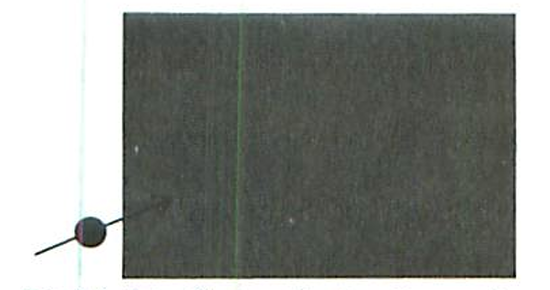
\includegraphics[width=.8\linewidth]{shot.png}
            \caption{The electron is shot into the gas}
            \label{fig:shot}
        \end{subfigure}
        \begin{subfigure}{.4\textwidth}
            \centering
            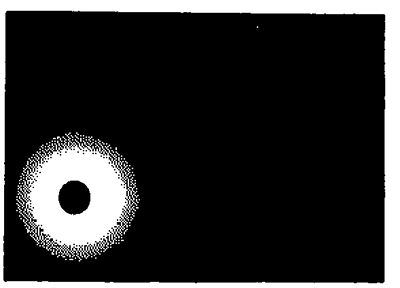
\includegraphics[width=.8\linewidth]{clothing.png}
            \caption{The electron creates holes as it moves along}
            \label{fig:clothing}
        \end{subfigure}
        \label{fig:propagates}
    \end{figure}
    Analogous to 
    \begin{equation}
        \highlight{\epsilon_{\text{self}} = \epsilon_{\text{quasi}} - \epsilon_{\text{bare}},}
    \end{equation}
    So $\Sigma$ is the difference between the quasi-particle and bare energies; an electron's "clothing."
\end{frame}

\begin{frame}
    \frametitle{\textcolor{caltechorange}{GW Approximation}}
    Hedin's equations\autocite{hedin_new_1965} define a self-consistent procedure, schematically\autocite{noauthor_frontiers_nodate} as
    \begin{figure}
        \centering
        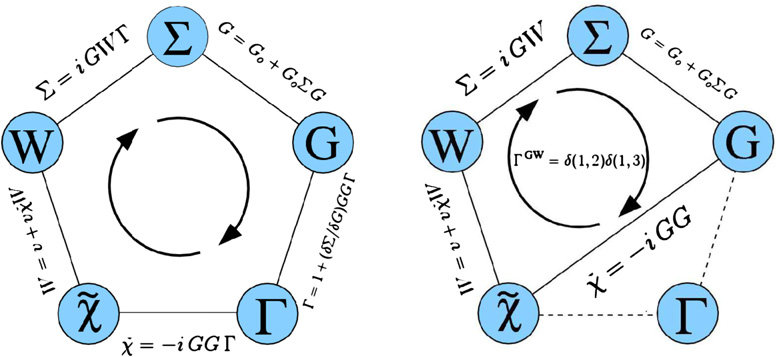
\includegraphics[width=\textwidth]{Left-panel-Graphical-representation-of-Hedins-equations-Right-panel-The-four-coupled.jpg}
        \label{fig:hedin}
    \end{figure}
    \pause
    \textcolor{red}{Where is the vertex function $\Gamma$ neglected?}\\
    \pause
    Right diagram constitutes the $GW$ approximation, whereas for the BSE we need to consider the left diagram.
\end{frame}

\begin{frame}
    \frametitle{\textcolor{caltechorange}{Bethe-Salpeter Equation}}
    \begin{itemize}
        \item \textcolor{red}{Why was linear response theory unable to describe excitons?}
        \pause
        \item Can define an electron-hole correlation function given by
        \begin{equation}
        \highlight{L\left(1,2 ; 1^{\prime}, 2^{\prime}\right)=-G_2\left(1,2 ; 1^{\prime}, 2^{\prime}\right)+G\left(1,1^{\prime}\right) G\left(2,2^{\prime}\right)}
        \end{equation}
        where we have defined a two-particle Green's function $G_2$.
        \pause
        \item Now we are able to describe the interaction between an electron and a hole because this is inherently a two-particle process.
    \end{itemize}
\end{frame}

\begin{frame}
    \frametitle{\textcolor{caltechorange}{Bibliography}}
    \printbibliography
\end{frame}

\end{document}
